\documentclass[10pt]{beamer}
\usepackage[utf8]{inputenc}
\usepackage{xeCJK}
\usepackage{graphicx}
\usepackage{mathtools}
\usepackage{utopia} % Utopia font
\usetheme{CambridgeUS}
\usecolortheme{dolphin}
\setbeamertemplate{headline}{}
\usepackage{tikz}
\usetikzlibrary{positioning}
\usepackage{pgfplots}
\usepackage{booktabs}
\usepackage{multirow}

% set colors
\definecolor{myNewColorA}{RGB}{126,12,110}
\definecolor{myNewColorB}{RGB}{165,85,154}
\definecolor{myNewColorC}{RGB}{203,158,197}
\setbeamercolor*{palette primary}{bg=myNewColorC}
\setbeamercolor*{palette secondary}{bg=myNewColorB, fg = white}
\setbeamercolor*{palette tertiary}{bg=myNewColorA, fg = white}
\setbeamercolor*{titlelike}{fg=myNewColorA}
\setbeamercolor*{title}{bg=myNewColorA, fg = white}
\setbeamercolor*{item}{fg=myNewColorA}
\setbeamercolor*{caption name}{fg=myNewColorA}

\usefonttheme{professionalfonts}
\usepackage{natbib}
\usepackage{hyperref}

% ------------------------------------------------------------
% Title metadata
% ------------------------------------------------------------
\titlegraphic{\includegraphics[height=1.5cm]{iitkgplogo.jpg}} 

\setbeamerfont{title}{size=\large}
\setbeamerfont{subtitle}{size=\small}
\setbeamerfont{author}{size=\small}
\setbeamerfont{date}{size=\small}
\setbeamerfont{institute}{size=\small}

\title[SLMs for Marine Hydrodynamics]{Small Language Models for Marine Hydrodynamics\\Problem Solving using RLPT}
\subtitle{Master's Thesis Final Presentation}
\author[R. Patil]{\textbf{Raghuveer Patil}\\Roll No.\ 21NA3AI42}
\institute[IIT Kharagpur]{Department of Artificial Intelligence\\Indian Institute of Technology Kharagpur\\[0.3cm]Supervisor: Prof.\ Prabhat Kumar Mishra}
\date[Apr 2026]{24 April 2026}

% ------------------------------------------------------------
% Section title pages
% ------------------------------------------------------------
\AtBeginSection[]{
  \begin{frame}
  \vfill
  \centering
  \begin{beamercolorbox}[sep=8pt,center,shadow=true,rounded=true]{title}
    \usebeamerfont{title}\insertsectionhead\par%
  \end{beamercolorbox}
  \vfill
  \end{frame}
}

% ------------------------------------------------------------
\begin{document}

% ============================================================
% Slide 1 — Title Page
% ============================================================
\frame{\titlepage}

% ============================================================
% Slide 2 — Outline
% ============================================================
\begin{frame}{Outline}
\large
\tableofcontents
\end{frame}

% ============================================================
\section{Introduction \& Motivation}
% ============================================================

% ============================================================
% Slide — Motivation
% ============================================================
\begin{frame}{Motivation: Why Domain-Specific SLMs?}
\large
\begin{itemize}
    \item Large Language Models (LLMs) excel at general reasoning but \textbf{underperform on specialised engineering tasks}.
    \vspace{0.25cm}

    \item Marine hydrodynamics requires:
    \begin{itemize}
        \item structured numerical reasoning,
        \item equation-based derivations,
        \item domain-specific formula selection.
    \end{itemize}
    \vspace{0.25cm}

    \item No publicly available QA datasets exist for graduate-level marine hydrodynamics.
    \vspace{0.25cm}

    \item \textbf{Key question:} Can a 3B-parameter SLM, trained with GRPO-based RL post-training, match a frontier LLM on domain-specific problems?
\end{itemize}
\end{frame}

% ============================================================
% Slide — Problem Statement
% ============================================================
\begin{frame}{Problem Statement}
\large
\begin{itemize}
    \item Three core challenges:
    \vspace{0.2cm}
    \begin{itemize}
        \item \textbf{No labelled datasets:} No benchmark exists for marine hydrodynamics QA.
        \vspace{0.15cm}
        \item \textbf{Numerical \& symbolic reasoning:} Problems require equation derivations, multi-step calculations.
        \vspace{0.15cm}
        \item \textbf{Evaluation difficulty:} Solutions must be verified against physical laws, not subjective judgment.
    \end{itemize}
    \vspace{0.3cm}

    \item \textbf{Central hypothesis:} GRPO-based RL post-training can bring a domain-specialised SLM to frontier LLM performance levels.
\end{itemize}
\end{frame}

% ============================================================
% Slide — Last Semester Recap
% ============================================================
\begin{frame}{Last Semester Recap}
\large
\begin{itemize}
    \item \textbf{Semester 1} (Nov 2025): Studied alignment methods under resource constraints on a T4 GPU (16 GB).
    \vspace{0.2cm}
    \begin{itemize}
        \item Implemented SFT, DPO, PPO, GRPO on Gemma-2B.
        \item PPO infeasible (OOM); DPO showed mode collapse.
        \item GRPO emerged as the most practical RL method.
    \end{itemize}
    \vspace{0.3cm}

    \item \textbf{Semester 2} (Apr 2026): Apply GRPO to a real engineering domain.
    \begin{itemize}
        \item Upgraded to NVIDIA H100 NVL (95 GB).
        \item Domain: Marine Hydrodynamics.
        \item Full pipeline: data generation $\to$ SFT $\to$ GRPO $\to$ evaluation.
    \end{itemize}
\end{itemize}
\end{frame}

% ============================================================
\section{Literature Review}
% ============================================================

% ============================================================
% Slide — Key Concepts
% ============================================================
\begin{frame}{Key Concepts}
\large
\begin{itemize}
    \item \textbf{SFT Objective:}
    \[
        \mathcal{L}_{\text{SFT}} = - \mathbb{E}_{(x,y)}[\log \pi_\theta(y\,|\,x)]
    \]

    \item \textbf{PPO Clipped Objective:}
    \[
        \mathcal{L}_{\text{PPO}} = 
        \min\!\left(
            r_\theta A,\;
            \text{clip}(r_\theta, 1-\epsilon, 1+\epsilon) A
        \right)
    \]

    \item \textbf{GRPO Group Advantage} (Shao et al., 2024):
    \[
        A_i^{(G)} = A_i - \frac{1}{|G|} \sum_{j \in G} A_j
    \]
\end{itemize}

\vspace{0.3cm}
{\small \textit{GRPO eliminates the value network $\Rightarrow$ lower VRAM, better stability for low-resource RL.}}
\end{frame}

% ============================================================
% Slide — Visualizing PPO vs GRPO
% ============================================================
\begin{frame}{PPO vs.\ GRPO: Why GRPO?}
\centering
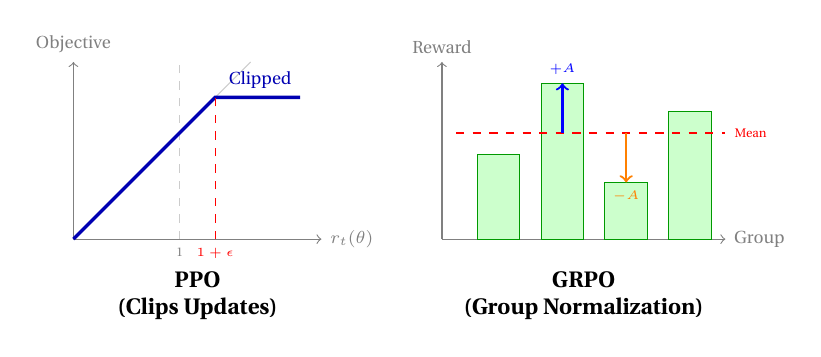
\begin{tikzpicture}[scale=0.9, transform shape] 

    % LEFT: PPO
    \draw[->, gray] (0,0) -- (3.5,0) node[right, font=\scriptsize] {$r_t(\theta)$};
    \draw[->, gray] (0,0) -- (0,2.5) node[above, font=\scriptsize] {Objective};
    \draw[dashed, gray!40] (1.5, 0) -- (1.5, 2.5);
    \node[below, font=\tiny, gray] at (1.5,0) {1};
    \draw[gray!40, thin] (0,0) -- (2.5,2.5);
    \draw[blue!70!black, very thick] (0,0) -- (2.0, 2.0) -- (3.2, 2.0);
    \draw[dashed, red] (2.0, 0) -- (2.0, 2.0);
    \node[below, font=\tiny, red] at (2.0,0) {$1+\epsilon$};
    \node[anchor=south east, font=\scriptsize, blue!70!black] at (3.2, 2.0) {Clipped};
    \node[font=\bfseries\small, align=center] at (1.75, -0.8) {PPO\\(Clips Updates)};

    % RIGHT: GRPO
    \begin{scope}[xshift=5.2cm] 
        \draw[->, gray] (0,0) -- (4.0,0) node[right, font=\scriptsize] {Group};
        \draw[->, gray] (0,0) -- (0,2.5) node[above, font=\scriptsize] {Reward};
        \foreach \x/\h in {0.5/1.2, 1.4/2.2, 2.3/0.8, 3.2/1.8} {
            \draw[fill=green!20, draw=green!60!black] (\x, 0) rectangle (\x+0.6, \h);
        }
        \draw[red, thick, dashed] (0.2, 1.5) -- (4.0, 1.5) node[right, font=\tiny] {Mean};
        \draw[->, blue, thick] (1.7, 1.5) -- (1.7, 2.2);
        \node[above, font=\tiny, blue] at (1.7, 2.2) {$+A$};
        \draw[->, orange, thick] (2.6, 1.5) -- (2.6, 0.8);
        \node[below, font=\tiny, orange] at (2.6, 0.8) {$-A$};
        \node[font=\bfseries\small, align=center] at (2.0, -0.8) {GRPO\\(Group Normalization)};
    \end{scope}

\end{tikzpicture}

\vspace{0.4cm}

\begin{columns}[t]
    \begin{column}{0.48\linewidth}
        \begin{block}{PPO}
            Requires policy, reference, \& value models. Memory-intensive.
        \end{block}
    \end{column}
    \begin{column}{0.48\linewidth}
        \begin{block}{GRPO}
            No value network. Group-normalized advantages. Single-GPU friendly.
        \end{block}
    \end{column}
\end{columns}
\end{frame}

% ============================================================
\section{Methodology}
% ============================================================

% ============================================================
% Slide — End-to-End Pipeline
% ============================================================
\begin{frame}{End-to-End Pipeline}
\begin{center}
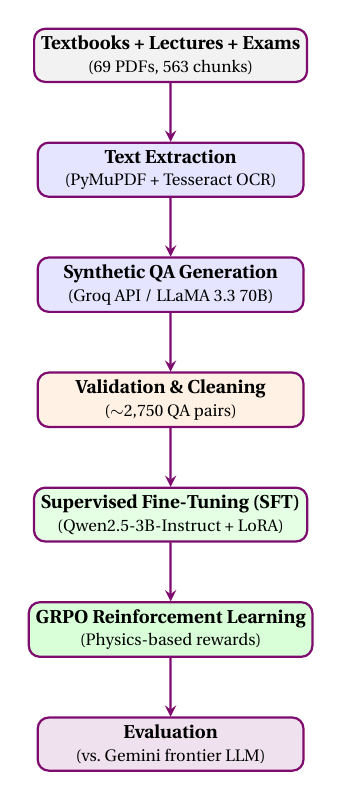
\begin{tikzpicture}[
    scale=0.75, transform shape,
    node distance=1.0cm,
    box/.style={
        draw=myNewColorA, thick, rounded corners, fill=white, align=center,
        font=\small\bfseries, minimum height=0.9cm, minimum width=4.5cm
    },
    arrow/.style={->, >=stealth, thick, color=myNewColorA}
]
    \node[box, fill=gray!10] (src) {Textbooks + Lectures + Exams\\{\normalfont\footnotesize (69 PDFs, 563 chunks)}};
    \node[box, fill=blue!10, below=of src] (extract) {Text Extraction\\{\normalfont\footnotesize (PyMuPDF + Tesseract OCR)}};
    \node[box, fill=blue!10, below=of extract] (qa) {Synthetic QA Generation\\{\normalfont\footnotesize (Groq API / LLaMA 3.3 70B)}};
    \node[box, fill=orange!10, below=of qa] (clean) {Validation \& Cleaning\\{\normalfont\footnotesize ($\sim$2,750 QA pairs)}};
    \node[box, fill=green!10, below=of clean] (sft) {Supervised Fine-Tuning (SFT)\\{\normalfont\footnotesize (Qwen2.5-3B-Instruct + LoRA)}};
    \node[box, fill=green!15, below=of sft] (grpo) {GRPO Reinforcement Learning\\{\normalfont\footnotesize (Physics-based rewards)}};
    \node[box, fill=myNewColorC!30, below=of grpo] (eval) {Evaluation\\{\normalfont\footnotesize (vs.\ Gemini frontier LLM)}};

    \draw[arrow] (src) -- (extract);
    \draw[arrow] (extract) -- (qa);
    \draw[arrow] (qa) -- (clean);
    \draw[arrow] (clean) -- (sft);
    \draw[arrow] (sft) -- (grpo);
    \draw[arrow] (grpo) -- (eval);
\end{tikzpicture}
\end{center}
\end{frame}

% ============================================================
% Slide — Data Sources
% ============================================================
\begin{frame}{Data Acquisition}
\large
\begin{itemize}
    \item \textbf{Source Materials:}
    \begin{itemize}
        \item Newman (1977) — \textit{Marine Hydrodynamics} (340 chunks)
        \item Faltinsen (1993) — \textit{Sea Loads} (156 chunks, OCR)
        \item MIT OCW 2.20 — 22 lectures, 25 problem sets, final exam
        \item MIT OCW 2.29 — 14 lecture notes (OCR)
        \item IIT Kharagpur NA20202 — 4 exam papers (OCR)
    \end{itemize}
    \vspace{0.2cm}
    \item \textbf{Total:} 69 PDFs $\to$ 563 text chunks (2.4 MB)
    \vspace{0.2cm}
    \item \textbf{Extraction:} PyMuPDF (digital PDFs) + Tesseract OCR (scanned PDFs)
\end{itemize}
\end{frame}

% ============================================================
% Slide — Synthetic QA Generation
% ============================================================
\begin{frame}{Synthetic QA Dataset Generation}
\large
\begin{itemize}
    \item Each chunk $\to$ Groq API (LLaMA 3.3 70B) $\to$ graduate-level QA pairs.
    \vspace{0.2cm}
    \item Three question types:
    \begin{itemize}
        \item Conceptual explanations
        \item Numerical problems (with worked solutions)
        \item Multiple-choice questions (MCQ)
    \end{itemize}
    \vspace{0.2cm}
    \item Every sample includes a \textbf{Chain-of-Thought (CoT)} reasoning trace.
    \vspace{0.2cm}
    \item \textbf{Final dataset:} $\sim$2,757 validated QA pairs.
    \vspace{0.2cm}
    \item Safeguards: API key rotation, checkpoint resumption, JSON extraction from free-form text.
\end{itemize}
\end{frame}

% ============================================================
% Slide — SFT Implementation
% ============================================================
\begin{frame}{Supervised Fine-Tuning (SFT)}
\large
\begin{columns}[t]
    \begin{column}{0.55\linewidth}
        \begin{itemize}
            \item \textbf{Base model:} Qwen2.5-3B-Instruct
            \item \textbf{Method:} LoRA adapters
            \item \textbf{Precision:} Float32 (BF16 caused NaN)
            \item \textbf{GPU:} NVIDIA H100 NVL (95 GB)
            \item \textbf{Epochs:} 3
            \item \textbf{Training time:} $\sim$9.4 minutes
        \end{itemize}
    \end{column}
    \begin{column}{0.43\linewidth}
        \begin{block}{LoRA Config}
            \footnotesize
            \begin{tabular}{ll}
                Rank ($r$) & 16 \\
                Alpha & 16 \\
                Dropout & 0.05 \\
                Targets & q, k, v, o\_proj \\
                Scaling & 1.0 \\
            \end{tabular}
        \end{block}
        \vspace{0.2cm}
        \begin{block}{SFT Results}
            \footnotesize
            \begin{tabular}{ll}
                Train loss & 0.9729 \\
                Eval loss & 0.9743 \\
                Token acc. & 77.43\% \\
            \end{tabular}
        \end{block}
    \end{column}
\end{columns}

\vspace{0.3cm}
\centering
{\small SFT provides domain knowledge and format structure, but numerical accuracy is only \textbf{27.60\%} $\Rightarrow$ motivates GRPO.}
\end{frame}

% ============================================================
% Slide — SFT-2 Corrected Pipeline
% ============================================================
\begin{frame}{SFT-2: Leak-Free Baseline}
\large
\begin{itemize}
    \item \textbf{Problem:} SFT-1 train/test split overlapped with GRPO evaluation set.
    \vspace{0.2cm}
    \item \textbf{Solution:} SFT-2 trained \emph{exclusively} on the GRPO training pool (2,206 records).
    \vspace{0.2cm}
    \item \textbf{Leak-free baseline:}
    \begin{itemize}
        \item Numerical accuracy: \textbf{27.60\%}
        \item MCQ accuracy: \textbf{71.82\%}
    \end{itemize}
    \vspace{0.2cm}
    \item This is the true starting point for measuring GRPO improvement.
\end{itemize}
\end{frame}

% ============================================================
% Slide — GRPO Reward Design
% ============================================================
\begin{frame}{GRPO: Reward Function Design}
\large
\begin{columns}[t]
    \begin{column}{0.55\linewidth}
        \textbf{Correctness Reward (Graded):}
        \[
            r_{\text{num}}(\hat{y}, y^*) = \begin{cases}
                1.0 & \leq 5\% \text{ error} \\
                0.7 & \leq 10\% \\
                0.4 & \leq 25\% \\
                0.15 & \leq 50\% \\
                0.0 & \text{otherwise}
            \end{cases}
        \]
        \vspace{0.2cm}
        \textbf{MCQ:} Binary (1.0 / 0.0)
    \end{column}
    \begin{column}{0.43\linewidth}
        \begin{block}{Format Reward}
            \footnotesize
            \begin{tabular}{lc}
                \toprule
                Component & Weight \\
                \midrule
                Reasoning section & 0.05 \\
                Final Answer line & 0.08 \\
                Reasonable length & 0.05 \\
                Structured steps & 0.02 \\
                \midrule
                Max total & $\sim$0.20 \\
                \bottomrule
            \end{tabular}
        \end{block}
        \vspace{0.1cm}
        {\footnotesize Format reward prevents the \textbf{zero-gradient problem}.}
    \end{column}
\end{columns}

\vspace{0.3cm}
\centering
$r_{\text{total}} = r_{\text{correctness}} + r_{\text{format}}$
\end{frame}

% ============================================================
% Slide — GRPO Training Runs Overview
% ============================================================
\begin{frame}{GRPO: Five Progressive Training Runs}
\large
\begin{itemize}
    \item \textbf{Run 1:} Binary reward + format reward; 1 epoch, $K=8$. \textit{max\_new\_tokens} not applied (TRL bug).
    \vspace{0.15cm}
    \item \textbf{Run 2:} Graded numerical reward; reduced format weights; completion logging.
    \vspace{0.15cm}
    \item \textbf{Run 3:} Extended training (2 epochs, $K=8$). Truncation bug corrupted 75--95\% of completions.
    \vspace{0.15cm}
    \item \textbf{Run 4:} Clean SFT-2 adapter; \textbf{truncation fix applied}. Clipped ratio $\approx 0$. First clean run.
    \vspace{0.15cm}
    \item \textbf{Run 5b:} Expanded LoRA ($r=32$, 7 target modules incl.\ MLP layers). \textbf{Full generation\_config patch}.
\end{itemize}
\end{frame}

% ============================================================
\section{Results \& Discussion}
% ============================================================

% ============================================================
% Slide — Cross-Run Comparison Table
% ============================================================
\begin{frame}{Cross-Run Performance Comparison}
\begin{center}
\footnotesize
\begin{tabular}{lcccc}
    \toprule
    \textbf{Stage} & \textbf{Num.\ Acc.} & \textbf{MCQ Acc.} & \textbf{max\_new\_tokens} & \textbf{Key Change} \\
    \midrule
    SFT-2 Baseline & 27.60\% & 71.82\% & --- & Leak-free baseline \\
    GRPO Run 1 & 38.01\% & 75.45\% & Not applied & Binary reward \\
    GRPO Run 3 & 39.37\% & \textbf{85.45\%} & Not applied & Extended training \\
    GRPO Run 4 & 38.46\% & \textbf{85.45\%} & Fixed (partial) & Truncation fix \\
    GRPO Run 5b & \textbf{38.91\%} & 80.00\% & Fixed (full) & LoRA $r=32$, MLP \\
    \midrule
    Gemini (frontier) & 37.10\% & 78.18\% & --- & LLM baseline \\
    \bottomrule
\end{tabular}
\end{center}

\vspace{0.3cm}
\large
\begin{itemize}
    \item Run 1 alone: \textbf{+10.41 pp} numerical accuracy over SFT-2.
    \item MCQ peaks at \textbf{85.45\%} (+13.63 pp over baseline).
    \item Numerical accuracy plateaus at $\sim$39\% across all clean runs.
\end{itemize}
\end{frame}

% ============================================================
% Slide — LLM Baseline Comparison
% ============================================================
\begin{frame}{SLM vs.\ Frontier LLM (Gemini)}
\begin{center}
\large
\begin{tabular}{lcc}
    \toprule
    \textbf{Model} & \textbf{Numerical Acc.} & \textbf{MCQ Acc.} \\
    \midrule
    SFT-2 Baseline (3B SLM) & 27.60\% & 71.82\% \\
    GRPO Run 5b (3B SLM) & \textbf{38.91\%} & \textbf{80.00\%} \\
    Gemini (frontier LLM) & 37.10\% & 78.18\% \\
    \midrule
    \textbf{SLM advantage} & \textbf{+1.81 pp} & \textbf{+1.82 pp} \\
    \bottomrule
\end{tabular}
\end{center}

\vspace{0.4cm}

\begin{block}{Key Finding}
The fine-tuned \textbf{3B SLM matches and marginally exceeds} the frontier LLM on both metrics, confirming that GRPO-based RL post-training successfully closes the SLM-to-LLM gap on this domain-specific benchmark.
\end{block}
\end{frame}

% ============================================================
% Slide — Numerical Graded Breakdown
% ============================================================
\begin{frame}{Numerical Accuracy: Graded Breakdown}
\begin{center}
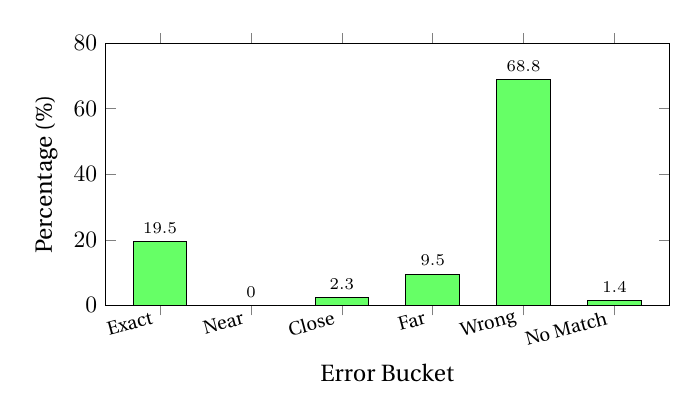
\begin{tikzpicture}[scale=0.85, transform shape]
\begin{axis}[
    ybar,
    bar width=0.8cm,
    width=10cm, height=5.5cm,
    xlabel={Error Bucket},
    ylabel={Percentage (\%)},
    symbolic x coords={Exact, Near, Close, Far, Wrong, No Match},
    xtick=data,
    x tick label style={font=\footnotesize, rotate=15, anchor=east},
    ymin=0, ymax=80,
    nodes near coords,
    nodes near coords align={vertical},
    every node near coord/.append style={font=\scriptsize},
    enlarge x limits=0.12,
    legend style={at={(0.97,0.97)}, anchor=north east, font=\scriptsize},
]
\addplot[fill=green!60] coordinates {
    (Exact,19.5) (Near,0.0) (Close,2.3) (Far,9.5) (Wrong,68.8) (No Match,1.4)
};
\end{axis}
\end{tikzpicture}
\end{center}

\vspace{0.2cm}
\large
\begin{itemize}
    \item \textbf{Bimodal distribution:} either exact ($\leq$5\% error) or completely wrong ($>$50\%).
    \item Failure is \textbf{formula selection}, not arithmetic imprecision.
\end{itemize}
\end{frame}

% ============================================================
% Slide — Shared Failure Pattern
% ============================================================
\begin{frame}{Shared Failure Pattern: SLM $\equiv$ Gemini}
\large
\begin{itemize}
    \item Both the fine-tuned SLM and Gemini exhibit an \textbf{identical error distribution}:
    \vspace{0.2cm}
    \begin{itemize}
        \item Zero failures with relative error $<5\%$.
        \item 95\% of failures have relative error $>20\%$ (wrong formula family).
    \end{itemize}
    \vspace{0.3cm}

    \item \textbf{Implication:} The $\sim$39\% numerical accuracy ceiling is a \textbf{data representation limitation}, not a model capacity issue.
    \vspace{0.3cm}

    \item The bottleneck is \textbf{diversity of worked numerical examples} in the training data, not model size or RL algorithm choice.
\end{itemize}
\end{frame}

% ============================================================
% Slide — Cumulative Progress
% ============================================================
\begin{frame}{Cumulative Progress Across All Stages}
\begin{center}
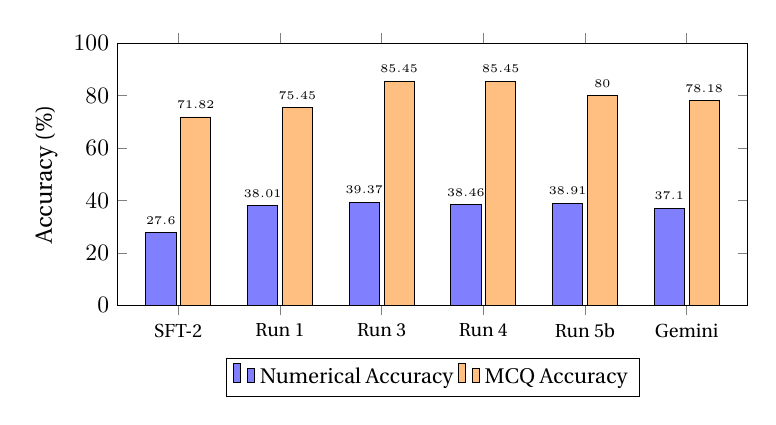
\begin{tikzpicture}[scale=0.85, transform shape]
\begin{axis}[
    ybar,
    bar width=0.45cm,
    width=11cm, height=5.5cm,
    ylabel={Accuracy (\%)},
    symbolic x coords={SFT-2, Run 1, Run 3, Run 4, Run 5b, Gemini},
    xtick=data,
    x tick label style={font=\footnotesize},
    ymin=0, ymax=100,
    legend style={at={(0.5,-0.2)}, anchor=north, legend columns=2, font=\small},
    enlarge x limits=0.12,
    nodes near coords,
    every node near coord/.append style={font=\tiny},
]
\addplot[fill=blue!50] coordinates {
    (SFT-2,27.60) (Run 1,38.01) (Run 3,39.37) (Run 4,38.46) (Run 5b,38.91) (Gemini,37.10)
};
\addplot[fill=orange!50] coordinates {
    (SFT-2,71.82) (Run 1,75.45) (Run 3,85.45) (Run 4,85.45) (Run 5b,80.00) (Gemini,78.18)
};
\legend{Numerical Accuracy, MCQ Accuracy}
\end{axis}
\end{tikzpicture}
\end{center}
\end{frame}

% ============================================================
\section{Error Analysis \& Debugging}
% ============================================================

% ============================================================
% Slide — BF16 NaN Investigation
% ============================================================
\begin{frame}{The BF16 NaN Gradient Investigation}
\large
\begin{itemize}
    \item<1-> \textbf{Symptom:} Every BF16 SFT run crashed at the same optimizer step with \texttt{grad\_norm: nan}.
    \vspace{0.2cm}

    \item<1-> \textbf{Perfect reproducibility} ruled out stochastic instability.
    \vspace{0.2cm}

    \item<2-> \textbf{7 failed hypotheses tested:}
    \begin{itemize}
        \item Special token init, embedding init, optimizer change, data cleaning, tag removal, batch reshuffling...
    \end{itemize}
    \vspace{0.2cm}

    \item<3-> \textbf{Root cause:} BF16's 7-bit mantissa accumulates rounding errors across multiple LoRA matrices during the optimizer step.
    \vspace{0.2cm}

    \item<3-> \textbf{Fix:} Switch to Float32 + reduce LoRA targets from 7 to 4 modules.
\end{itemize}
\end{frame}

% ============================================================
% Slide — Truncation Bug
% ============================================================
\begin{frame}{The Truncation Bug}
\large
\begin{itemize}
    \item<1-> \textbf{Problem:} \texttt{max\_new\_tokens} was silently dropped by \texttt{GRPOConfig} (TRL 1.0.0).
    \vspace{0.2cm}

    \item<1-> Model defaulted to $\sim$256 tokens $\Rightarrow$ completions truncated before ``Final Answer:'' $\Rightarrow$ \textbf{false zero rewards}.
    \vspace{0.2cm}

    \item<2-> \textbf{Evidence:} \texttt{completions/clipped} ratio rose from 0.05 to 0.75--0.95 during training.
    \vspace{0.2cm}

    \item<3-> \textbf{Resolution (two-stage):}
    \begin{enumerate}
        \item Run 4: \texttt{model.generation\_config} fallback (partial fix).
        \item Run 5b: Patch \texttt{trainer.generation\_config} directly after construction (complete fix).
    \end{enumerate}
\end{itemize}
\end{frame}

% ============================================================
% Slide — Zero Gradient Problem
% ============================================================
\begin{frame}{The GRPO Zero-Gradient Problem}
\large
\begin{itemize}
    \item \textbf{Symptom:} \texttt{grad\_norm = 0} for majority of early training steps.
    \vspace{0.2cm}

    \item \textbf{Cause:} All $K$ completions received the same binary reward $\Rightarrow$ zero advantage $\Rightarrow$ zero gradients.
    \vspace{0.3cm}

    \item \textbf{Three-part fix:}
    \begin{enumerate}
        \item Increased $K$ from 4 to 8 (more within-group variance).
        \item Added sampling diversity: temperature=0.8, top-$p$=0.95.
        \item \textbf{Non-binary format reward} (most impactful fix).
    \end{enumerate}
\end{itemize}
\end{frame}

% ============================================================
% Slide — Error Summary Table
% ============================================================
\begin{frame}{Error Resolution Summary}
\begin{center}
\footnotesize
\begin{tabular}{lll}
    \toprule
    \textbf{Component} & \textbf{Error} & \textbf{Resolution} \\
    \midrule
    SFT & BF16 NaN at step 50 & Float32; LoRA $\to$ 4 modules \\
    SFT & SFTTrainer API change & Migrated to SFTConfig + ChatML \\
    GRPO & Zero gradient norm & Format reward + sampling diversity \\
    GRPO & \texttt{max\_new\_tokens} not applied & \texttt{generation\_config} fallback \\
    GRPO & Groq API rate limiting & Disabled LLM judge in training \\
    Verifier & IndexError on empty answer & Empty-list guard \\
    All & OSError 28 (disk full) & Redirected to \texttt{/tmp} \\
    \bottomrule
\end{tabular}
\end{center}
\end{frame}

% ============================================================
\section{Discussion \& Key Insights}
% ============================================================

% ============================================================
% Slide — Key Insights
% ============================================================
\begin{frame}{Key Insights}
\large
\begin{enumerate}
    \item \textbf{SFT $\neq$ numerical precision.} 77.4\% token accuracy, but only 27.60\% numerical accuracy.
    \vspace{0.2cm}

    \item \textbf{GRPO excels at MCQ improvement.} 71.82\% $\to$ 85.45\% (+13.63 pp).
    \vspace{0.2cm}

    \item \textbf{Numerical accuracy plateaus at $\sim$39\%} regardless of LoRA capacity, training duration, or configuration.
    \vspace{0.2cm}

    \item \textbf{Implementation correctness matters as much as algorithm choice.} The truncation bug silently corrupted the reward signal.
    \vspace{0.2cm}

    \item \textbf{GRPO closes the SLM-to-LLM gap.} 3B SLM $\geq$ frontier LLM on this domain benchmark.
\end{enumerate}
\end{frame}

% ============================================================
% Slide — Limitations
% ============================================================
\begin{frame}{Limitations}
\large
\begin{itemize}
    \item \textbf{Conceptual evaluation not performed} (Groq API rate limits prevented LLM-as-judge).
    \vspace{0.2cm}
    \item \textbf{Truncation bug} corrupted numerical reward signal in Runs 1--3.
    \vspace{0.2cm}
    \item \textbf{Numerical ceiling at $\sim$39\%} — formula-selection limitation driven by insufficient diversity of worked examples.
    \vspace{0.2cm}
    \item \textbf{Single GPU} — limited hyperparameter search.
    \vspace{0.2cm}
    \item \textbf{Dataset size} — $\sim$2,750 QA pairs may not cover full formula diversity.
\end{itemize}
\end{frame}

% ============================================================
\section{Conclusion \& Future Work}
% ============================================================

% ============================================================
% Slide — Conclusion
% ============================================================
\begin{frame}{Conclusion}
\large
\begin{itemize}
    \item<1-> \textbf{Central question answered affirmatively:}
    \begin{center}
        \textit{GRPO-based RL post-training can bring a 3B SLM to frontier LLM performance on domain-specific engineering problems.}
    \end{center}

    \vspace{0.2cm}

    \item<1-> Numerical accuracy: 27.60\% $\to$ \textbf{38.91\%} (SLM) vs.\ 37.10\% (Gemini).

    \vspace{0.2cm}

    \item<1-> MCQ accuracy: 71.82\% $\to$ \textbf{85.45\%} (SLM) vs.\ 78.18\% (Gemini).

    \vspace{0.2cm}

    \item<2-> The shared failure pattern confirms: \textbf{bottleneck is data, not model scale}.

    \vspace{0.2cm}

    \item<2-> \textbf{Data augmentation is more impactful than scaling model size} for this class of problems.
\end{itemize}
\end{frame}

% ============================================================
% Slide — Future Work
% ============================================================
\begin{frame}{Future Work}
\large
\begin{itemize}
    \item<1-> \textbf{Numerical Data Augmentation (SFT3-NumAug):}
    \begin{itemize}
        \item Formula-focused worked examples to break the 39\% ceiling.
    \end{itemize}

    \vspace{0.2cm}

    \item<1-> \textbf{Conceptual Evaluation:}
    \begin{itemize}
        \item Activate LLM-as-judge pipeline once API access is stable.
    \end{itemize}

    \vspace{0.2cm}

    \item<1-> \textbf{VLLM Integration:}
    \begin{itemize}
        \item High-throughput RL rollouts; more epochs, larger $K$.
    \end{itemize}

    \vspace{0.2cm}

    \item<2-> \textbf{Curriculum-Based GRPO Training:}
    \begin{itemize}
        \item Progress from simple to complex numerical problems.
    \end{itemize}

    \vspace{0.2cm}

    \item<2-> \textbf{Rejection Sampling SFT:}
    \begin{itemize}
        \item Mine correct completions from GRPO logs for additional SFT.
    \end{itemize}

    \vspace{0.2cm}

    \item<2-> \textbf{Broader LLM Comparison:}
    \begin{itemize}
        \item GPT-4 class models, other open-source LLMs.
    \end{itemize}
\end{itemize}
\end{frame}

% ============================================================
% Thank You
% ============================================================
\section*{Acknowledgement}

\begin{frame}
    \vspace{1.0cm}
    \centering
    \textcolor{myNewColorA}{\Huge \textbf{Thank you!}}

    \vspace{0.5cm}
    {\large Questions?}
\end{frame}

% ------------------------------------------------------------
\end{document}
